%======================================================================
\chapter{Background}
\label{chap:bg}
%======================================================================

The first augmented reality system can be dated back to 1960s~\cite{sutherland1968,johnson2010, yuen2011}. It employed a see-through Head-Mounted Display (HMD). The HMD was tracked by a mechanical tracker and an ultrasonic tracker. However, only simple wireframes could be drawn and overlaid on the user's view due to the lack of computing capacity at that time~\cite{sutherland1968}. In 1992, Boeing~\cite{caudell1992} had already leveraged AR technology to assist their workers in assembling wire bundles.

The research and development for AR have gone on over the past five decades. The use of augmented reality technology has been explored in various fields, e.g. education, training, tourism, gaming, health, 
% Should be overviews
safty, etc~\cite{freitas2008,schrier2005,billinghurst2001}.
Freitas and Campos~\cite{freitas2008} developed an educational system using AR technology. The system teaches 2nd grade-level concepts, such as the means of transportation and types of animals. The system tracks a marker and superimposes the 3D models on the real-time video feed shown to the whole class. Experiments show that the nature of game-base learning of this system helps increase motivation among students~\cite{freitas2008}.
Schrier~\cite{schrier2005} developed a historic role-play game at a real site. The participants are assigned to a specific historic role and interact with virtual roles with a GPS-enabled mobile device.
Billings Hurst et al.~\cite{billinghurst2001} implemented a more interactive and realistic way of reading books. If the users look at the pages through a handheld AR display, they see 3D models appearing out of the pages.

There exist many reviews of implementations and progress in augmented reality applications~\cite{billinghurst2002,regenbrecht2005,zhou2008,lee2012}.
Billinghurst and Kato~\cite{billinghurst2002} focused on collaborative AR applications and demonstrated examples that allow people to view or change the same virtual models.
Regenbrecht et al.~\cite{regenbrecht2005} showed ten AR applications in various fields which make cutting edge progress at that time.
Zhou et al.~\cite{zhou2008} summarize the papers published on ISMAR from 1997 to 2007 in an statistical way. They focus on analyzing the frequency and percentage of citations of each topic involved in augmented reality applications.
Lee~\cite{lee2012} discussed the areas that augmented reality technology has been used in and identify how it can be used in each area.

In this section, we focus on the use of augmented reality technology in training.
But before that, we first review the literature in general AR area.

\section{General Scenarios}
\label{sec:bg:gs}

After reviewing recent progress in this area, we propose a new methodology of categorizing the AR applications. We categorize them into two categories in terms of interactive targets: real objects and virtual objects. Fig.~\ref{fig:category} shows two examples, where the left one shows that a trainee is interacting with a real object, and the right one depict that a trainee is interacting with a virtual object. When interacting with a real object, the overlaid virtual ones act as an instruction that guides the trainee through the process.

\begin{figure}
	\centering
	\subfigure[Interact with real objects]{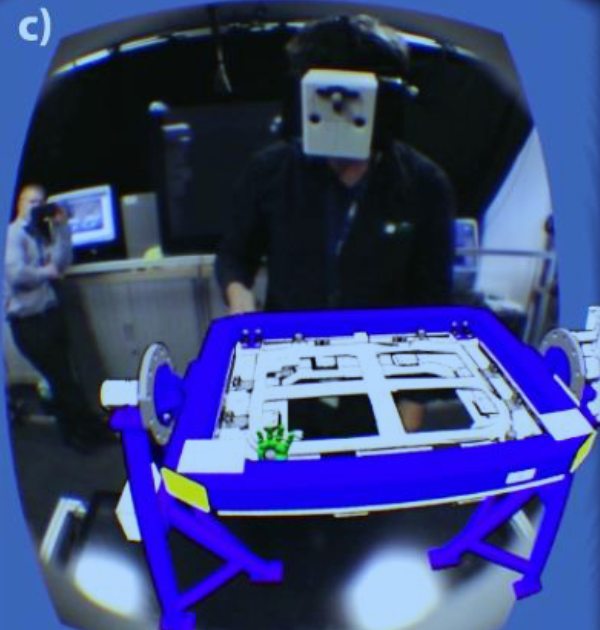
\includegraphics[width=0.35\columnwidth]{figures/category2.png}}
	\subfigure[Interact with virtual objects]{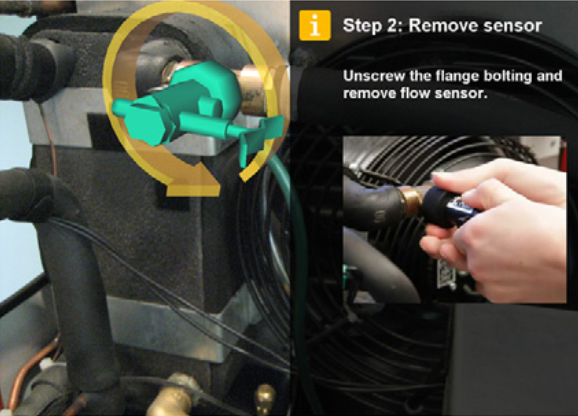
\includegraphics[width=0.51\columnwidth]{figures/category1.png}}
	\caption{Two categories of augmented reality training scenarios according to which objects people interact with.}
	\label{fig:category}
\end{figure}

\subsection{Virtual Objects}
\label{sec:bg:gs:vo}

In the framework depicted in~\cite{nakajima2003}, the camera captures the images of a participant standing in front of a blue screen. The participant uses a "wand" to interact with a virtual environment, where the "wand" can be a finger, a fire extinguisher or other things we have seen in normal life. There is no marker needed to recognize the position and orientation of the "wand".
Luo et al.~\cite{luo2005} developed an AR-based therapy application that was designed for post-stroke finger extension rehabilitation. The application involves both therapists and the patients. During the rehabilitation, the patients need to wear a head-mounted display and an orthosis. The virtual objects prepared by the therapist are mixed with the patient's hand and displayed on the head-mounted display. When the patient is trying to grasp or release the virtual object, the on-site therapist adjusts the assistance provided by the orthosis.
Leblanc et al.~\cite{leblanc2010} compared an AR training method with the traditional methods in the field of straight laparoscopic colorectal skills acquisition training. The traditional methods cost much higher than the the AR training method since it uses human cadavers. They conclude that simulator training followed by cadaver training can appropriately integrate simulators into the learning curve and maintain the benefits of both training methodologies.
Nishino et al. present a Japanese calligraphy training system to teach learners how to write better characters~\cite{nishino2011}. It allows the learners to watch and feel the writing techniques of an instructor. More specifically, the training system displays a virtual brush and enables the learners to intuitively master instructor's motor skills through the sense of touch with a haptic device.
Gonzalez-Franco et al.~\cite{gonzalez-franco2016} developed an approach for training in complex manufacturing scenarios, where the virtual objects are projected into real scenes without their real counterparts. The trainers operate on the virtual objects with a wand to teach the trainees.
% This sentence is not needed
In this use case, the interactive targets are the virtual objects.

The methods in this category are usually applied on the fields where the cost or risk of real hands-on experience is too high. For example, a surgeon could use AR to learn how to perform open-heart surgery without risking patients' lives.

\subsection{Real Objects}
\label{sec:bg:gs:ro}

In engineering, especially in the field of machine maintenance and repairing, the cost of real hands-on experience is relatively low, but the complexity of the target is very high. In this kind of scenarios, people often use augmented reality technology to show virtual objects as a guide.

Hincapi� et al.~\cite{hincapie2011} demonstrated an AR-based training process to perform maintenance on the body of the RV-10 aircraft. The system overlays virtual objects onto real objects as an instruction. Trainees need to work on the RV-10 aircraft component based on the instructions.
Webel et al.~\cite{webel2011,webel2013} proposed a framework for assembly and maintenance training. The trainees operate on a real machine, while the instructions are shown by overlaying a virtual machine on the real one. In this work, the interactive targets are the real objects, while the virtual ones are shown as the instruction.
Mohr et al.~\cite{mohr2015} present a system which automatically transfers printed technical documentation, such as handbooks, to three-dimensional augmented reality. The proposed system identifies the most frequent forms of instructions found in printed documentation, such as image sequences, explosion diagrams, textual annotations and arrows indicating motion.
Zhu et al.~\cite{zhu2017} aimed to develop a novel registration and tracking technique to establish a navigation system based on augmented reality for maxillofacial surgery. They use a marker to track the relationship between the virtual image and the real object for displaying inferior alveolar nerve bundles in maxillofacial surgery.

AR training scenarios typically involve interacting with objects in the real world, so most of AR training applications fall into the ``Real Objects'' category.
It could be very complex for an AR training system. The modules involved can be categorized into six categories~\cite{wang2016}, i.e., video capture, image analysis and processing, tracking process, interaction handling, instruction information management and rendering. In this article, we target in two of them, i.e., instruction information management and rendering.

\section{Training Scenarios}
\label{sec:bg:ts}

Among various fields of augmented reality, we are especially interested in AR's application in training.
Compared with traditional training approaches, trainers trained with AR demonstrate less unsolved errors~\cite{gavish2015_evaluating}.
Recently, a lot of efforts are paid on the use of AR in training area, especially during the past 10 years.

After reviewing the literature on this area, we categorize the existing works into 3 categories: guidance design, authoring and feedback. The reason why we use the three categories is that guidance is how the trainees accept instructions, authoring is where the guidance comes from while feedback is how the trainees' operations are evaluated and corrected.

Caudell and Mizell~\cite{caudell1992} have proposed the first implementation of a classic AR assembly system by combining head position sensing and real world registration with the HMD, such that a computer-produced diagram, containing pertinent information, can be superimposed and stabilized on a specific position on a real-world object.
Since then, many AR training guidance applications have emerged.
Henderson and Feiner developed a framework to assist conducting military routine maintenance tasks inside an armored vehicle turret~\cite{henderson2009}. The experiment shows that use of AR increases the precision of component locating by 56\% compared with the use of traditional untracked head-up displays (HUDs) and speeds up the task by 47\% compared with standard computer monitors.
Crescenzio et al.~\cite{crescenzio2011} implemented an AR-based maintenance tool for daily inspections of the Cessna C.172P, an airplane often used by flight schools. It superimposes digital replicas of parts and subparts or graphical symbols to attract the operator's attention and guide the technicians through a task. It uses a markerless, feature-based method for HMD registration. What is more interesting is that they also provide an authoring tool for new training material generation. By leveraging the CAD models and existing scanning tools, a trainer can generate new training materials without the knowledge of programming. However, it still requires a lot of efforts to scan real scenes for locating the virtual objects in the real scenes.

In order to be more robust, the applications above are designed as task-specific, i.e. not suited for a wide range of different tasks. Practical authoring solution is an popular research topic which has been sought after by the researchers.
Wang et al.~\cite{wang2010} developed an authoring tool for AR-based examinations. Providing 3D models involved in exam questions, the application generates the AR content and stores it in a separate file that can be shared, edited or imported into an AR interface.
Petersen and Stricker~\cite{petersen2012} reported proof-of-concept systems to create interactive AR manual automatically (for assembly, maintenance, etc.) by segmenting video sequences and live-streams of manual workflows into the comprising single tasks.
However, authoring an AR guidance could be very time-consuming using those tools.
Anderson et al.~\cite{anderson2013} proposed a movement training application that is equipped with a human motion recording tool. They record people's movements and present them in an augmented reality mirror, and the users can see their mirror image as well as the targeting movements in the mirror and follow those movements.
Bhattacharva and Winer~\cite{bhattacharya2015} also presented a method which uses a novel method to capture product assembly steps performed by a user with a depth+RGB camera.
However, they are still not real-time authoring tools, since the content need to be prepared or captured before the training.

Feedback plays an important role in AR training.
There are two types of feedback mechanisms among existing works.
The methods in one type use a intelligent system to evaluate the users' actions.
Nguyen~\cite{kruger2015} proposed an approach to compute the positions of each part of the worker's body with captured input depth images, and analyze the ergonomic scores.
Westerfield et al.~\cite{westerfield2013,westerfield2015} integrated the intelligent tutoring systems (ITSs) with AR interfaces to provide customized instruction to each trainee.
The methods in another type allow supervisors to review and evaluate the task activity performed by the trainees.
Re and Bordegoni~\cite{re2014} presented a monitor system for training, such that supervisors could check the assembly/maintenance activity from a remote display and provide feedback to the users whenever necessary.
To the author's knowledge, there is no existing work that focuses on real-time feedback that could be integrated into the AR training system.

As discussed above, most of the AR training systems are presented as interactive guidances that guide the user through a fixed series of steps.
There are a few issues that need more attention from researchers. First, pre-designed guidances, no matter they leverage an intelligent schema or not, are not suited for a wide range of different tasks, especially for the complex ones, since they are always designed as task-specific. Second, lack of collaboration between the trainer and the trainees limits the use of AR training methods in complex tasks, because the trainer is not able to get real-time feedbacks from the trainees.

In this article, we propose a collaborative AR training framework that is not a traditional guidance-like system.
Compared to the existing AR training platforms, the proposed platform has three advantages: 1) It does not require a pre-defined guidance, which makes it suitable to complex tasks; 2) It allows the trainer to collect feedbacks from the trainees during the training process in real-time; 3) It works with mobile devices without powerful graphics capacity.

